\newpage
\section{Prinsipiell løsning}
\label{prinsipiellLoesning}

%Her kan du skrive om prinsipiell løsning

Et signal inneholder ofte flere frekvenser, dette gjelder også for lyd. Ettersom lydsignalet som er gitt ut er en musikkinspilling så kan man forvente å finne frekvenser fra 20Hz til 20kHz \cite{Frq_in_audio} i lydsignalet. Det er derfor viktig å kunne filtrere ut de frekvensene som ikke er ønsket. Dette kan gjøres ved hjelp av et system som vist i Figur \ref{fig:fig1}. Dette systemet kan moddeleres med likningen \ref{eq:01eq1}. \cite{Tek_notat}

\begin{figure}[!h]
	\centering
	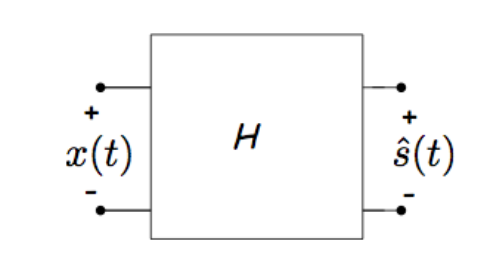
\includegraphics[width=0.5\textwidth]{Bilder/Overordnetsystem.png}
	\caption{Overordnet system}
	\label{fig:fig1}
\end{figure}

\begin{equation}
	\label{eq:01eq1}
	\begin{split}
		x(t) = \hat{s}(t) + \omega(t).
	\end{split}
\end{equation}

For å få til ønsket effekt så burde man benytte seg av et båndstopp filter som fejerner støy på en bestemt frekvens. Siden vi skal blokere ut samme frekvens hele tiden så kan vi lage et tidsinvariant filter. Det finnes mange forskjellige båndstop filterdesign, både aktive og passive, noen populære varianter er: \href{https://www.falstad.com/afilter/circuitjs.html?cct=$+1+0.000005+5+50+5+50%0A%25+0+4540.3852025771785%0Ar+928+256+928+432+0+50%0A170+784+256+752+256+2+20+4000+5+0.1%0AO+928+256+992+256+0%0Aw+784+208+784+256+0%0Aw+864+208+864+256+0%0Ag+864+432+864+448+0%0Ag+928+432+928+448+0%0Ac+784+256+864+256+0+0.000004593296450259804+0%0Ac+864+352+864+432+0+1.7108344904994753e-7+0%0Al+784+208+864+208+0+0.0008554172452497378+0%0Al+864+256+864+352+0+0.022966482251299023+0%0AB+784+128+864+528+3+Box%0Aw+864+256+928+256+0%0A}{Butterworth}-, \href{https://en.wikipedia.org/wiki/Chebyshev_filter}{Chebyshev}- og \href{https://www.sciencedirect.com/topics/engineering/elliptic-filters}{Elliptic} båndstoppfiltere, disse er relativt koplekse og krever flere komponeneter enn det som er tilgjengelig. I tillegg finnes det et veldig enkelt RLC filter som kan brukes til å filtrere ut støy på en bestemt frekvens. Dette filteret er veldig enkelt å lage og krever kun 3 komponenter. Dette filteret er et 2. ordens filter som består av en kondensator, en spole og en motstand som vist i figur \ref{fig:fig2}

\begin{figure}[!h]
	\centering
	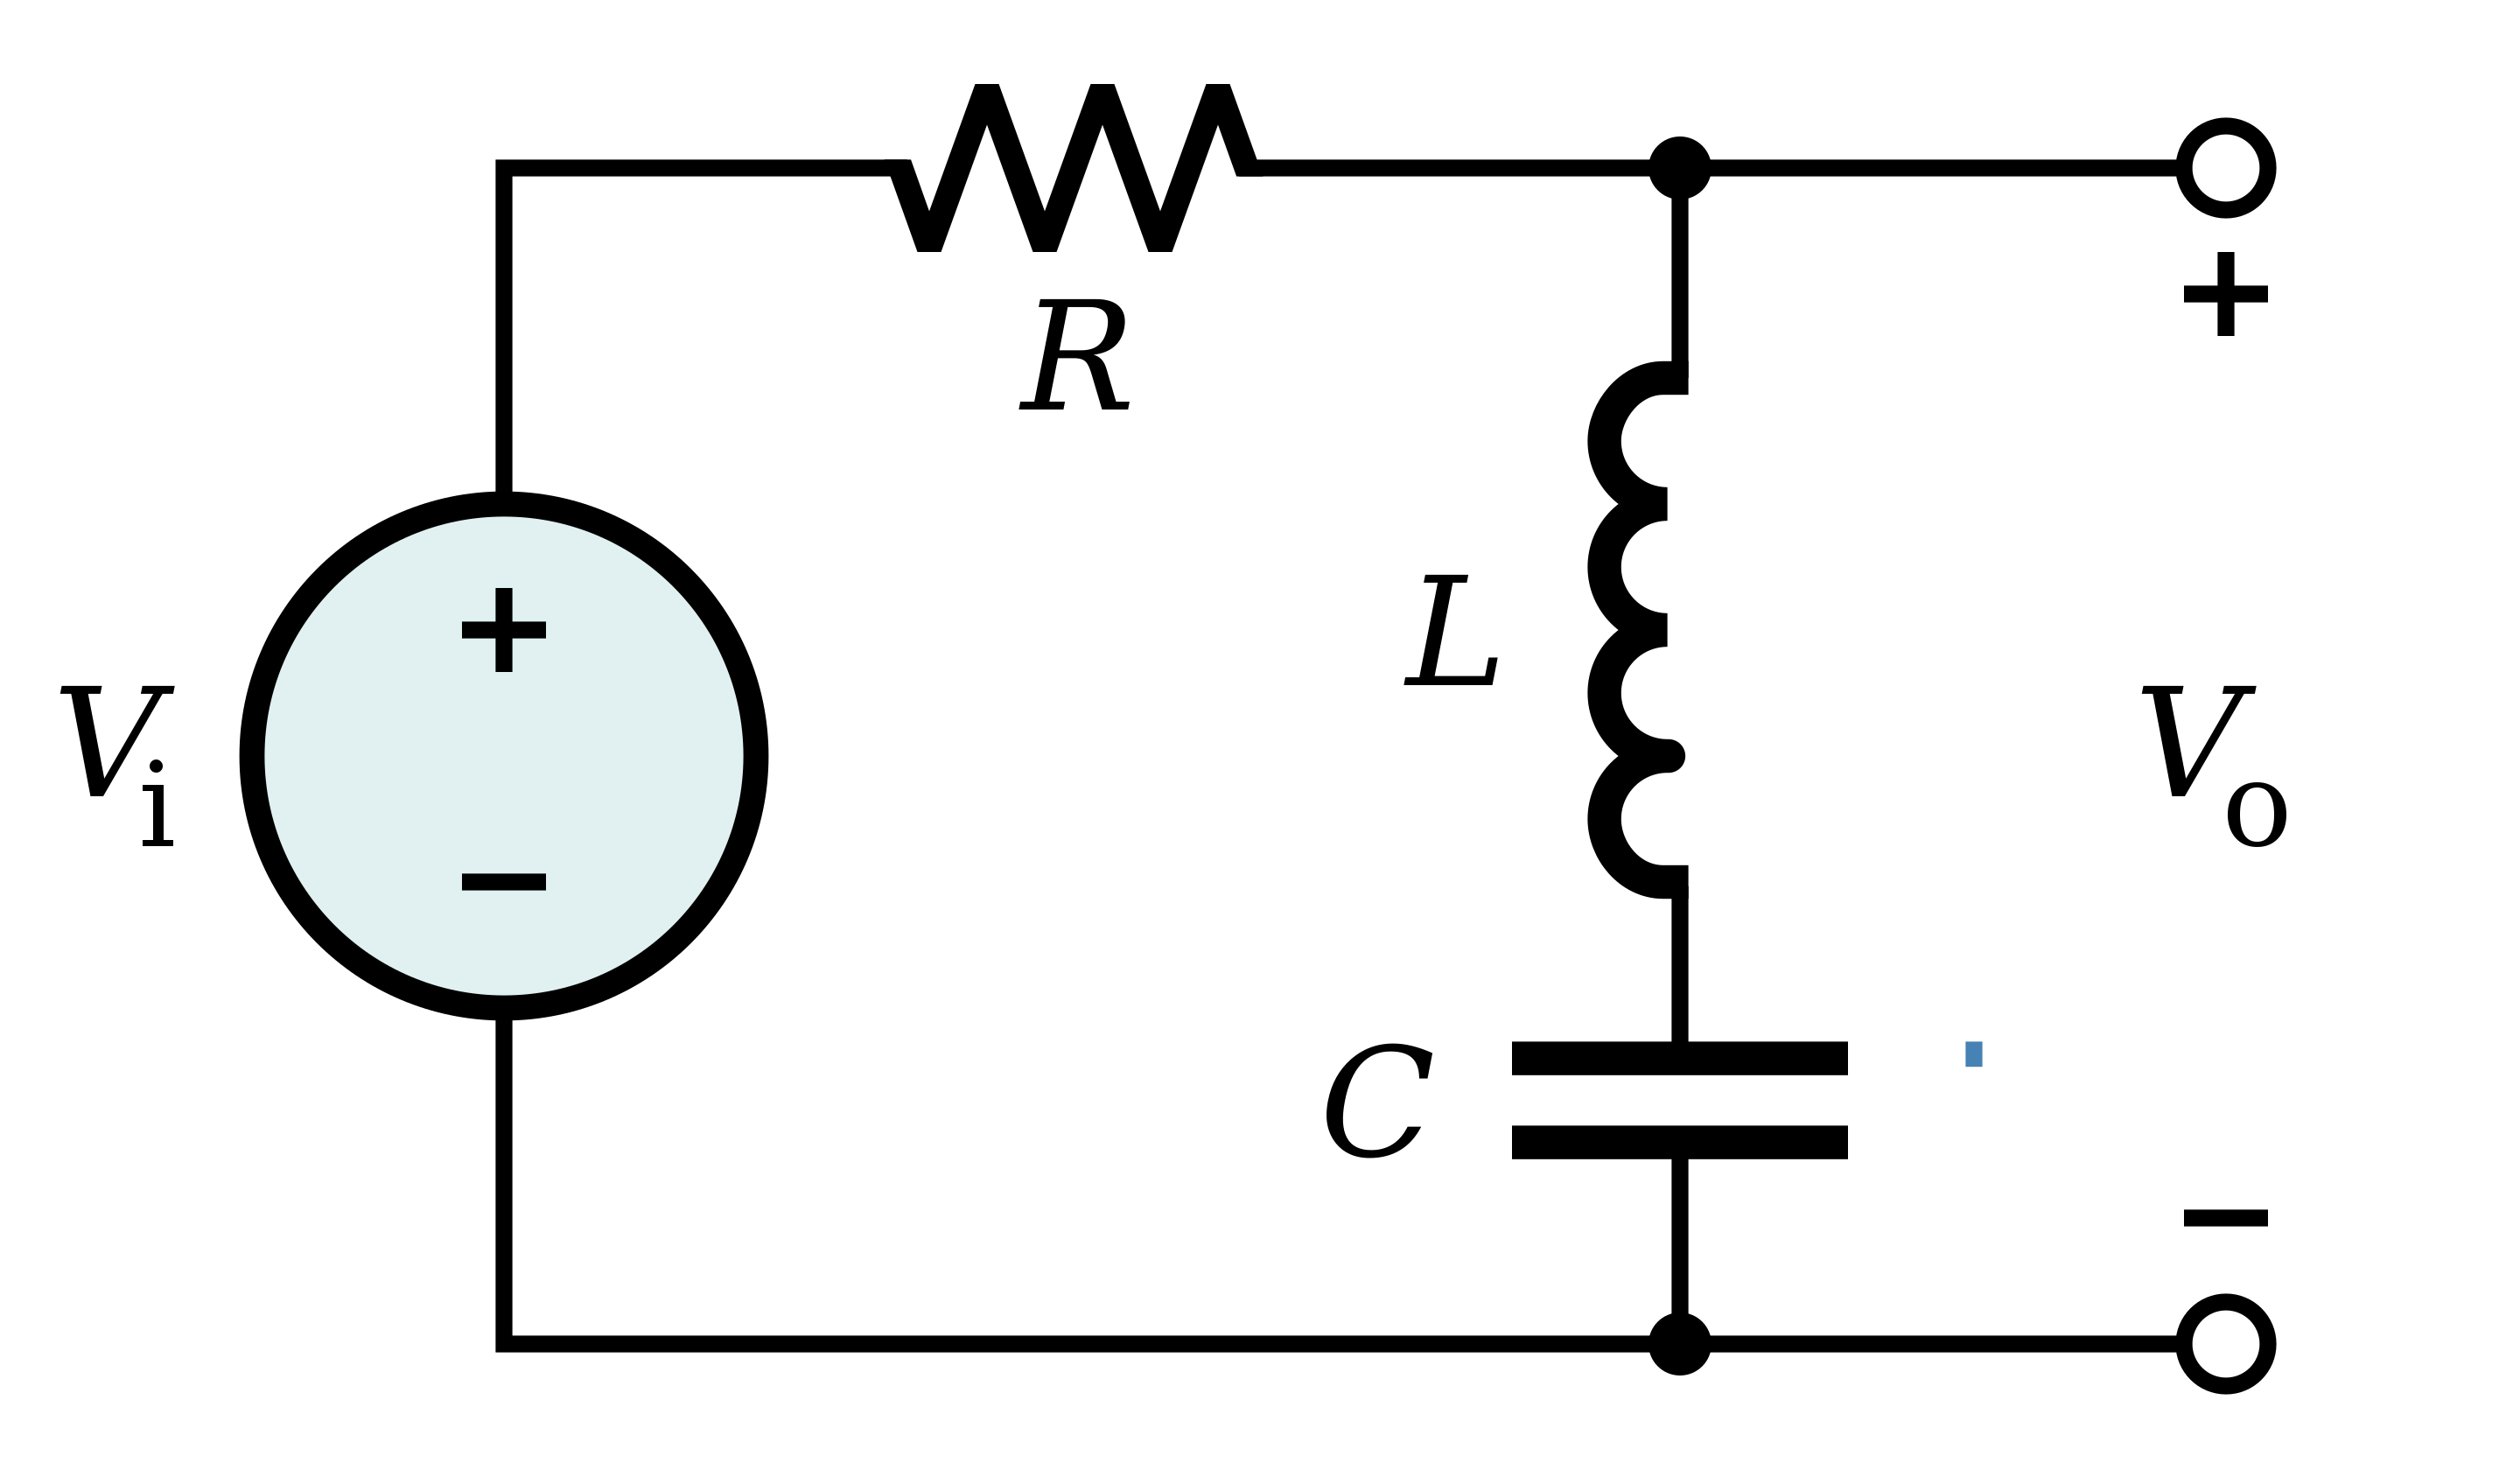
\includegraphics[width=0.5\textwidth]{Bilder/Band-Reject_Filter.svg.png}
	\caption{RLC filter}
	\label{fig:fig2}
\end{figure}

